\documentclass[a4paper,
fontsize=11pt,
%headings=small,
oneside,
numbers=noperiodatend,
parskip=half-,
bibliography=totoc,
final
]{scrartcl}

\usepackage[babel]{csquotes}
\usepackage{synttree}
\usepackage{graphicx}
\setkeys{Gin}{width=.4\textwidth} %default pics size

\graphicspath{{./plots/}}
\usepackage[ngerman]{babel}
\usepackage[T1]{fontenc}
%\usepackage{amsmath}
\usepackage[utf8x]{inputenc}
\usepackage [hyphens]{url}
\usepackage{booktabs} 
\usepackage[left=2.4cm,right=2.4cm,top=2.3cm,bottom=2cm,includeheadfoot]{geometry}
\usepackage{eurosym}
\usepackage{multirow}
\usepackage[ngerman]{varioref}
\setcapindent{1em}
\renewcommand{\labelitemi}{--}
\usepackage{paralist}
\usepackage{pdfpages}
\usepackage{lscape}
\usepackage{float}
\usepackage{acronym}
\usepackage{eurosym}
\usepackage{longtable,lscape}
\usepackage{mathpazo}
\usepackage[normalem]{ulem} %emphasize weiterhin kursiv
\usepackage[flushmargin,ragged]{footmisc} % left align footnote
\usepackage{ccicons} 
\setcapindent{0pt} % no indentation in captions

%%%% fancy LIBREAS URL color 
\usepackage{xcolor}
\definecolor{libreas}{RGB}{112,0,0}

\usepackage{listings}

\urlstyle{same}  % don't use monospace font for urls

\usepackage[fleqn]{amsmath}

%adjust fontsize for part

\usepackage{sectsty}
\partfont{\large}

%Das BibTeX-Zeichen mit \BibTeX setzen:
\def\symbol#1{\char #1\relax}
\def\bsl{{\tt\symbol{'134}}}
\def\BibTeX{{\rm B\kern-.05em{\sc i\kern-.025em b}\kern-.08em
    T\kern-.1667em\lower.7ex\hbox{E}\kern-.125emX}}

\usepackage{fancyhdr}
\fancyhf{}
\pagestyle{fancyplain}
\fancyhead[R]{\thepage}

% make sure bookmarks are created eventough sections are not numbered!
% uncommend if sections are numbered (bookmarks created by default)
\makeatletter
\renewcommand\@seccntformat[1]{}
\makeatother

% typo setup
\clubpenalty = 10000
\widowpenalty = 10000
\displaywidowpenalty = 10000

\usepackage{hyperxmp}
\usepackage[colorlinks, linkcolor=black,citecolor=black, urlcolor=libreas,
breaklinks= true,bookmarks=true,bookmarksopen=true]{hyperref}
\usepackage{breakurl}

%meta
%meta

\fancyhead[L]{Redaktion LIBREAS\\ %author
LIBREAS. Library Ideas, 40 (2021). % journal, issue, volume.
\href{https://doi.org/10.18452/23802}{\color{black}https://doi.org/10.18452/23802}
{}} % doi 
\fancyhead[R]{\thepage} %page number
\fancyfoot[L] {\ccLogo \ccAttribution\ \href{https://creativecommons.org/licenses/by/4.0/}{\color{black}Creative Commons BY 4.0}}  %licence
\fancyfoot[R] {ISSN: 1860-7950}

\title{\LARGE{Editorial \#40: Dekolonisierung}}% title
\author{Redaktion LIBREAS} % author

\setcounter{page}{1}

\hypersetup{%
      pdftitle={Editorial \#40: Dekolonisierung},
      pdfauthor={Redaktion LIBREAS},
      pdfcopyright={CC BY 4.0 International},
      pdfsubject={LIBREAS. Library Ideas, 40 (2021)},
      pdfkeywords={Bibliothek, Dekolonisierung, library, decolonization},
      pdflicenseurl={https://creativecommons.org/licenses/by/4.0/},
      pdfcontacturl={http://libreas.eu},
      baseurl={https://doi.org/10.18452/23802},
      pdflang={de},
      pdfmetalang={de}
     }



\date{}
\begin{document}

\maketitle
\thispagestyle{fancyplain} 

%abstracts

%body
{\par \centering \textbf{Wir widmen diese Ausgabe Engelbert Plassmann (1935--2021).}\par}

{\par \centering ***\par}

Anders als Museen, die sich in den vergangenen Jahren zunehmend mit
kolonialem Raubgut in ihren Sammlungen auseinandersetzen, haben sich
Bibliotheken bislang nur wenig mit dem befasst, was mit dem Begriff
\enquote{Dekolonisierung} verbunden werden kann. Wir verstehen darunter
die bewusste Auseinandersetzung mit den Nachwirkungen und
Einschreibungen kolonialer Muster in die Institution, ihre Organisation
und ihre Arbeitsprozesse sowie der unrechtmäßigen Vereinnahmung von
Kulturgütern. Dies mag daran liegen, dass beispielsweise geraubte Bücher
im wissenschaftlichen Diskurs lange als Domäne der Provenienzforschung
im Kontext der Aufarbeitung nationalsozialistischer Verbrechen
betrachtet wurden. Zudem gestaltet sich die Auseinandersetzung mit der
oft unterschwelligen Reproduktion von Rassismen schwierig, da die
entsprechenden Deutungs- und Abwertungsmuster stark -- oft untrennbar --
mit europäischen Denktraditionen verwoben sind und wissenschaftliche
Herangehensweisen unmittelbar davon abgeleitet wurden, teils auch noch
werden. Der bei der Dekolonisierung schwerste Schritt ist hier
tatsächlich der erste Schritt, nämlich das Infragestellen des eigenen
Denkens.

Die Relativierung und Dekonstruktion vermeintlicher
Selbstverständlichkeiten, das Aufbrechen und die kritische
Differenzierung von Traditionen und das aktive Zurücktreten aus den
eigenen Privilegien ist für Institutionen wie auch für Individuen eine
Herausforderung, teils auch eine Zumutung. Mitunter legt sie eigene
Verstrickungen frei. Es ist ein permanentes Konfrontiertwerden mit
unangenehmen Wahrheiten. Zugleich ist der Schritt unumgänglich, und zwar
bereits bevor der Anspruch erhoben wird, dass das westliche Verständnis
von Humanität endlich eingelöst hätte, was seit der Aufklärung als
Versprechen -- nämlich allgemeine, gleiche und freie Menschlichkeit für
alle -- von Anfang an in ihm lag.

Die Herausforderung der Dekolonisierung liegt im umfassenden und
unvermeidlich radikalen Anspruch dieses Ansatzes. Fragt man, welche
Bereiche davon betroffen sind, so lautet die Antwort: alle.

\hypertarget{dekolonisierung-und-bibliotheken}{%
\section{Dekolonisierung und
Bibliotheken}\label{dekolonisierung-und-bibliotheken}}

In Bibliotheken begegnen uns eurozentrische Geisteshaltungen in allen
Tätigkeiten und Positionierungen, aber auch in den Strukturen,
technischen Anwendungen und systemimmanenten Mechanismen. Dies lässt
sich am Beispiel einer subjektiv angenommenen Überlegenheit des Eigenen
und einer daraus resultierenden vermeintlichen Unterlegenheit des
Anderen auf verschiedenen Ebenen in unterschiedlichen Ausprägungen
veranschaulichen: nämlich dem Bestandsaufbau. Ein einfacher Blick in
einen Bibliothekskatalog offenbart, dass, aus unterschiedlichen Gründen,
bevorzugt Literatur aus dem \enquote{Globalen Norden} angekauft wird.
Dies wird besonders dann gravierend, wenn sich diese Literatur mit
Themen des \enquote{Globalen Südens} befasst. Dazu kommt, dass Normdaten
und Klassifikationen aus einer bestimmten Perspektive erschließen und
damit diese zugleich stabilisierend fortsetzen.

Bereits das Erkennen der entsprechenden Problemstellen, die daraus
resultieren, dass Institutionen und das Berufsbild über lange Strecken
nicht divers genug waren, wäre ein erheblicher Fortschritt. In der
Verknüpfung mit den Idealbildern westlicher Wissenschaft und
Wissenskulturen positionierten sich Bibliotheken in epistemologischen
Machtkämpfen eindeutig, unterstützten den Ausschluss nicht-hegemonialer
Wissenstraditionen und -produktionen in Ordnungssystemen. Man will
unterstellen, dass dies oft unwillkürlich und ohne Vorsatz geschah. Aber
es geschah. Und der Vorsatz wird dann sichtbar, wenn auf der
diskurspolitischen Ebene die Weigerung zum Beispiel der Verwendung
integrativer Sprache offenbar wird.

\hypertarget{zu-unserer-positionierung}{%
\section{Zu unserer
Positionierung}\label{zu-unserer-positionierung}}

Die Gestaltung dieser LIBREAS-Ausgabe fiel uns aus verschiedenen Gründen
weniger leicht, als wir es gewohnt sind. Andererseits fügten sich einige
glückliche Umstände ineinander.

Im Oktober 2020 traten unsere späteren Gastredakteurinnen Sandra Sparber
und Gabriele Slezak mit uns in Kontakt und berichteten von einem Wiener
Seminar am Institut für Afrikawissenschaften zum Thema Dekolonisieren
von Bibliotheksbeständen, das bereits zum dritten Mal in Folge
stattgefunden hatte. Wir äußerten Interesse an der Veröffentlichung
einiger Seminarbeiträge und daraus entstand die Idee zu einem zweiten
Schwerpunkt für die Ausgabe 39 (Roboter und Automatisierung)
aufzurufen.\footnote{\url{https://libreas.wordpress.com/2021/01/27/call-for-papers-libreas-ausgabe-39-2-schwerpunkt-dekolonisierung/}}
Dieser Call for Papers sowie einige jetzt veröffentlichte Beiträge
entstanden zudem im Kontext des zweisemestrigen LIBREAS-Projektseminars
am Institut für Bibliotheks- und Informationswissenschaft an der
Humboldt-Universität zu Berlin, bei dem sich Redaktionsmitglieder mit
sehr engagierten Studierenden dem Diskurs zu nähern versuchten und
Fachexpertise einholten. Daraufhin erreichten uns sehr unterschiedliche
Textangebote, die uns lange beschäftigten, sodass wir beschlossen eine
eigene Schwerpunktausgabe zu entwickeln. Zahlreiche gemeinsame virtuelle
Treffen mit Wien und mit Publizierenden der jetzigen Ausgabe sowie der
im September 2021 auf dem LIBREAS-Blog veröffentlichte Call for
Networking\footnote{\url{https://libreas.wordpress.com/2021/09/03/call-for-networking-einladung-zur-vernetzung-und-austausch-zum-thema-dekolonialisierung-und-antirassismus-in-wissenschaftlichen-bibliotheken/}}
zeugen von unser aller Bemühen, unsere redaktionellen Tätigkeiten,
Lehre, Diskursproblematisierung und Netzwerkarbeit unter einen Hut zu
bekommen.

Die Erfahrung zeigt: zum einen steckt die Zusammenführung
unterschiedlicher Initiativen, Forschungen und Debatten im
deutschsprachigen Raum am Anfang. Dies ist sogar gravierender, als wir
zunächst vermuteten. Dekolonisierung im Bibliothekswesen ist ein sich
entfaltendes Diskursphänomen, das jedoch weitgehend auf dem Stand
wechselseitiger Versicherung einer generellen Notwendigkeit bleibt.
Initiativen außerhalb des Bibliothekswesens waren zugleich schwer für
uns erreichbar. Im Ergebnis ist diese Ausgabe primär dem Versuch
verpflichtet, einen ersten Überblick über diverse Zugänge und
Ansatzpunkte zu verschaffen. Andererseits, und entscheidender, wurde uns
als Redaktionsteam schnell bewusst, dass wir selbst einer vermeintlich
homogenen Gruppe von weiß gelesenen, akademisierten Menschen im
Bibliotheksumfeld angehören. Wir waren daher vor allem gefordert, uns
mit den blinden Flecken der eigenen Wahrnehmung auseinanderzusetzen. Die
theoretisch-reflexive Beschäftigung mit dem Thema reicht nur bis zu
einem bestimmten Punkt. Ja, sogar bereits die Tatsache, dass wir uns
einfach so hinsetzen und anmaßen können, das Thema mit einem Stapel
Bücher zu bearbeiten, ist ein Zeichen des Privilegs. Konsequenter wäre
gewesen, sich jenseits der Literatur noch weiter mit Betroffenen
und/oder Aktivist*innen auszutauschen. Auch hier bliebe die Frage: Wer
spricht, wer übersetzt, wer setzt das Thema? Klar ist: Die
Deutungshoheit zum Thema Dekolonisierung sollte eigentlich von anderen
kommen, als von uns. Es ließ sich für dieses Mal kaum einlösen, weshalb
die Ausgabe nur als ein Herantasten zu bewerten sein kann.

Wir sind also in einer Unlösbarkeit gefangen. Das zu akzeptieren, ist
wahrscheinlich die erste Lektion, die das Thema Dekolonisierung für alle
weiß gelesenen, akademisch qualifizierten Bibliotheks- und
Informationswissenschaftler*innen bereithält. Zusammengenommen ist es
das bisschen, was wir bis hierhin zum Diskurs beitragen können.

Diese Schwerpunktausgabe kann somit nur einen Versuch darstellen, den
Bereich des kolonialen Erbes in Bibliotheken einer breiteren Debatte
zugänglich zu machen. Sie soll dazu anregen, sich mit den Strukturen im
eigenen bibliothekarischen Setting auseinanderzusetzen, vertraute Muster
zu hinterfragen und neue Praktiken jenseits sozial (ab)wertender
Dimensionen zu finden. Sehr gern laden wir ein, dazu auch fernab eines
Schwerpunktes Beiträge im Themenkomplex Dekolonisierung für nächste
Ausgaben beizutragen.

\begin{figure}
\centering
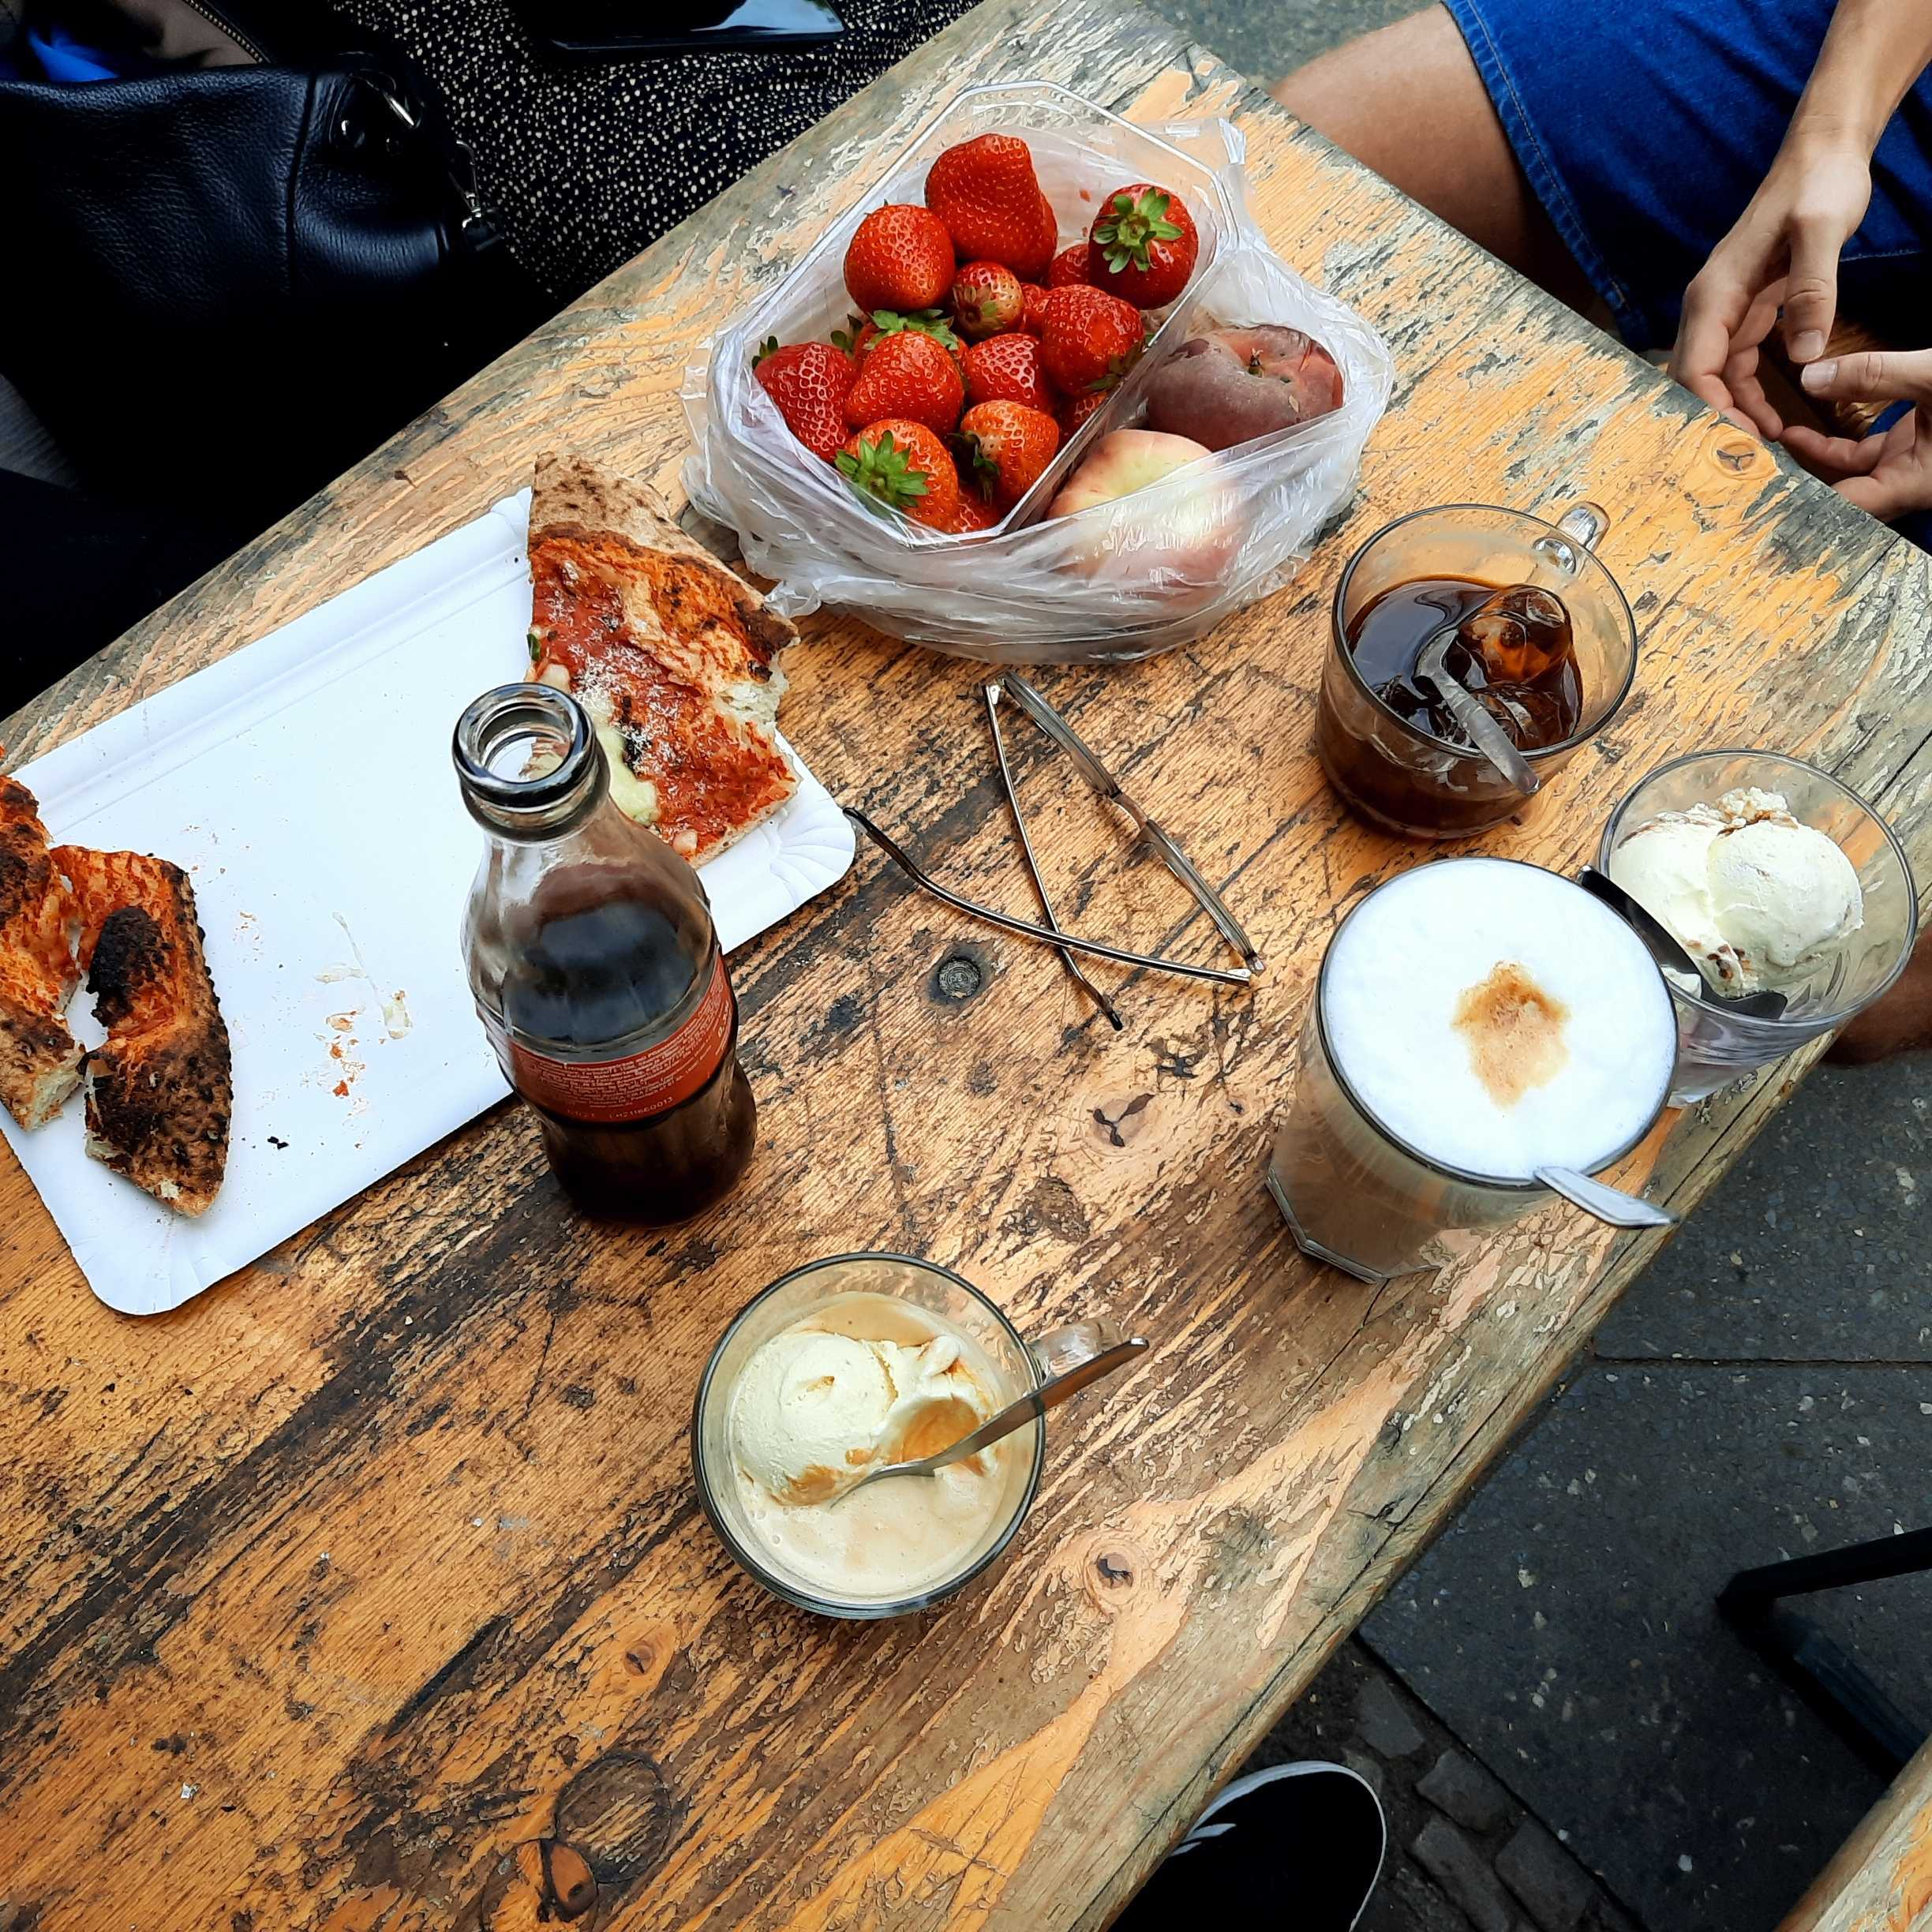
\includegraphics{img/img1.jpg}
\caption{Redaktionsorte XIX -- Berlin-Neukölln, Sommer 2021}
\end{figure}

\hypertarget{zu-den-einzelnen-beitruxe4gen}{%
\section{Zu den einzelnen
Beiträgen}\label{zu-den-einzelnen-beitruxe4gen}}

Einen Einblick, welche Auswirkungen \emph{Whiteness} in einer
rassifizierten und klassierenden Gesellschaft wie jener von Brasilien
hat, gibt das von Valentina Gonçalves de Toledo geführte Interview mit
der Bibliotheks- und Informationswissenschaftlerin Franciéle Carneiro
Garcês da Silva. Sie beschreibt, wie eine \emph{policy of whitening}
indigene(s) und afro-brasilianische(s) Wissen und Kultur nahezu
traditionell verdrängt und unterdrückt. Für das Bibliothekswesen
bedeutet diese Ignoranz gegenüber der Wissensproduktion ganzer
Bevölkerungsgruppen und epistemischer Kulturen auch, dass eine im
\enquote{Globalen Norden} etablierte Wissenschaftskultur zum Maß aller
Dinge wurde und weiterhin ist.

Mit Verweis auf ihre Dissertation \enquote{The Privilege to Select}
stellt Nora Schmidt \enquote{Überlegungen zur Dekolonialisierung
wissenschaftlicher Bibliotheken in Europa} an. Sie beschreibt diese
Überlagerung lokaler Wissensproduktionssysteme des \enquote{Globalen
Südens} durch jene des \enquote{Globalen Nordens} als Ausdruck von
Kolonialität. Diese Fortschreibung der Dominanz des \enquote{Globalen
Nordens} führt im Bereich des Wissenschaftssystems zu Ungleichheiten auf
verschiedenen Ebenen. Bibliotheken tragen aufgrund gängiger Praktiken
wie etwa der Medienauswahl, dem Ranking von Ergebnissen in Suchmaschinen
oder unreflektierter biblio- und szientometrischer Aktivitäten dazu bei.
Abschließend stellt die Autorin eine Liste mit Vorschlägen konkreter
Maßnahmen zur Dekolonialisierung von Bibliotheken zur Verfügung.

Der Text von Paula Herm bietet, basierend auf ihrer Masterarbeit von
2019, zuerst eine Einführung in das Thema Postkolonialität mit
systemtheoretischer Sicht und bezieht dies dann auf Strukturen von
Bibliotheken, Archiven und Museen im deutschsprachigen Raum. Dabei zeigt
sie, dass es zwar Ansätze, aber noch keine breite Auseinandersetzung mit
dem Thema gibt und deshalb auch noch keine wirkliche Praxis von
Bibliotheken, sich dekolonial zu engagieren. Gleichzeitig ist eine
solche Auseinandersetzung aber möglich.

Yvonne Schürer thematisiert, warum sie es als Bibliothekarin (in
Sachsen) wichtig findet, sich überhaupt mit dem
\enquote{Dekolonialisieren} zu befassen. Der Beitrag zeigt auch, dass es
immer möglich ist, die ersten Schritte zu tun und dafür nicht notwendig,
gleich den gesamten theoretischen Überbau durchzuarbeiten.

Fragen nach der \enquote{Ethik des Digitalisierens} stellt Matthias
Harbeck. Er umreißt das Problem der Massendigitalisierung kolonialer
Inhalte in Hinblick auf Zugänglichkeit beziehungsweise Barrieren und der
möglichen Reproduktion von Machtverhältnissen. Der Autor beschreibt die
Herangehensweise und Umsetzung in einem seit 2013 von der Deutschen
Forschungsgemeinschaft geförderten Digitalisierungsprojekt durch den
Fachinformationsdienst Sozial- und Kulturanthropologie.

Birgit Kramreither berichtet, wie die Fachbereichsbibliothek Kultur- und
Sozialanthropologie der Universität Wien in Aufklärungsprojekten wie
Ausstellungen ihrer kolonialen Vergangenheit begegnet. In Hinblick auf
die Aufarbeitung sensibler Materialien im Rahmen des Ethnographischen
Datenarchivs (EDA) thematisiert sie etwa die Bedeutung digitaler Objekte
auch im Kontext von Rückstellungen kolonialen Raubguts. Die Autorin
führt auch vor Augen, wie notwendig ein verantwortungsvoller Umgang mit
Metadaten ist, um Personen durch Offenlegung nicht einer
Gefährdungssituation auszusetzen.

Moritz Strickert widmet sich den Problemen und Möglichkeiten
kontrollierten Vokabulars am Beispiel der Gemeinsamen Normdatei (GND).
Er hält fest, dass normierte Begriffe und ein nicht auf Universalität
angelegter Anspruch, welcher zwangsläufig zu Lücken im Ordnungssystem
führt, zu einem Mangel an Diversität und zu eingeschränkter
Repräsentation führen. In Linked-Data-Ansätzen wie der
Anschlussfähigkeit von community-generierten Vokabularen oder dem Mapping
mit fremdsprachigen Erschließungsinstrumentarien, erkennt der Autor
Möglichkeiten, eurozentrischen Ausprägungen der GND zumindest in
Ansätzen entgegenzuwirken.

Gabriele Slezak et al.~fassen die Aktivitäten der Wiener C3-Bibliothek
für Entwicklungspolitik zusammen. Dort beschäftigt man sich seit 2018
mit den eigenen kolonialen Beständen. Neben Seminaren an der Universität
Wien (aus denen auch die Beiträge von Elisa Frei und Sandra Sparber
hervorgingen) initiiert man Workshops zur Vermittlung kritischer
Informationskompetenz für Schüler*innen und arbeitet mit Personen
verschiedener Communitys zusammen.

2019 löste die Neuauflage des österreichischen Kinderbuchs
\enquote{Hatschi Bratschis Luftballon} eine auf Wien beschränkte Debatte
in den sozialen Medien aus. Das 1904 erstmals erschienene Buch, das in
Österreich als Klassiker gilt, basiert auf einer an sich rassistischen
Erzählung mit entsprechenden Illustrationen. Elisa Frei hat die
öffentliche Auseinandersetzung zum Anlass genommen und Interviews mit
Bibliothekar*innen geführt. Sie wollte herausfinden, weshalb
Bibliotheken die Neuauflage angekauft haben und welches
Problembewusstsein und gegebenenfalls welche Strategien hinsichtlich
rassistischer Inhalte bestehen.

Sandra Sparber verortet Dimensionen sozialer Abwertung in Form von
\emph{Othering,} dem Abgrenzen der vermeintlich eigenen Gruppe von
anderen Personen(gruppen), auf drei Ebenen des Bibliotheksbestandes --
nämlich innerhalb der Disziplin beziehungsweise dem Sammelgebiet, der
Wissensordnung und der einzelnen Werke. Im Rahmen einer historischen
Bestandsanalyse untersucht sie eine missionswissenschaftliche
Sondersammlung und leitet daraus Handlungsempfehlungen für zukünftige
Projekte ab.

\emph{\enquote{La condition de la liberté n'est pas d'être gouverné par
l'histoire, mais de la réécrire au (temps) présent.}}\footnote{Felwine
  Sarr ; Bénédicte Savoy: \emph{Restituer le patrimoine african}. Paris:
  Philippe Rey / Seuil, 2018: 139.}

{\par \centering ***\par}

Ihre / Eure Redaktion LIBREAS und die Gastredakteurinnen Gabriele
Slezak und Sandra Sparber

(Berlin, Hannover, Göttingen, Lausanne, München, Wien)

%autor

\end{document}
